%!TEX root = ../template.tex
%%%%%%%%%%%%%%%%%%%%%%%%%%%%%%%%%%%%%%%%%%%%%%%%%%%%%%%%%%%%%%%%%%%%
%% chapter2.tex
%% NOVA thesis document file
%%
%% Chapter with the template manual
%%%%%%%%%%%%%%%%%%%%%%%%%%%%%%%%%%%%%%%%%%%%%%%%%%%%%%%%%%%%%%%%%%%%

\typeout{NT FILE chapter2.tex}%

\chapter{Related Work}
\label{cha:related_work}
In this chapter we examine some topics and techniques that are vital for the work proposal
presented in this document. These topics include \nameref{sec:gossip_protocols}, a dissemination
method, \nameref{sec:wireless_sensor_networks} and of particular interest for applications
devoted to tracking animals, the \nameref{sec:existing_commercial_solutions},
where it is discussed some of the existing collars with similar purpose as the proposed to be
develop during this dissertation, and, lastly, the \nameref{sec:cows}, that explains how the cows behave in herds,
their diet, and its consequences to the plant communities.


\section{Gossip Protocols}
\label{sec:gossip_protocols}
Gossip protocols \cite{Demers1987}, also known as epidemic protocols, were first proposed as
highly scalable and resilient approaches to implement reliable dissemination of information
\cite{Bakhshi2007, Friedman2009, Kermarrec2007}. For a protocol to be considered reliable it
must deliver the messages to all the nodes in the network, even if there are network omissions
or node failures \cite{Leitao2012}.

Subsequentially these protocols were used to resolve many other problems, such as failure detection,
data aggregation, overlay topology construction and many more\cite{Montresor2017}.

\subsection{History and Overview}
\label{subsec:gossip_history_overview}
Gossip protocols, as the name indicates, were created based on how rumors are propagated in
social groups \cite{Leitao2007}. In a gossip protocol, nodes in a network send the information, randomly, to
other nodes in the same network, similar to how a rumor is spread between members in a social
group.

These protocols are based on every participant propagating their messages collaboratively
throughout all the members of their group.

This process starts when a node desires to propagate some piece of information to the other
members of his network. This node will send his message to \textit{t} nodes, chosen randomly,
(\textit{t} being a parameter called \textit{fanout}, which is better explained in the
Section~\ref{subsubsec:gossip_parameters}). When the receiving nodes receives the message for
the first time, they will do the same as the previous node and resend the message to
\textit{t}, randomly chosen nodes. If a node receives the same message twice, it will discard
it. When this happens, which may occur quite often since the nodes are unaware of which nodes
have already received a message, there is communication redundancy, which while undesirable,
serves the purpose of making omissions (e.g. messages that are not correctly received).

However, since neither node knows who has received each message and who has sent a
message to whom, each node will have to keep a log of all messages that it has already
received, to avoid delivering it multiple times to the application and avoid messages
to circulate in the network forever.


\subsubsection{Parameters}
\label{subsubsec:gossip_parameters}
Gossip protocols have parameters that should be taken in consideration when using this
class of protocols. The most relevant ones are \cite{Leitao2012}:
\begin{description}
      \item[Fanout:] represents the number of nodes that each node will propagate its message
            to, in each propagating step of the message.
      \item[Maximum Rounds:] represents how many times a message can be retransmitted. Each
            message has a value of rounds associated to it, starting with zero and adding one
            unit every time a node retransmits the message to a neighbour. When this value
            reaches a maximum round value the message is no longer retransmitted and is simply
            dropped.
\end{description}

Both these parameters demonstrated a clear trade-off between reliability and redundancy. If
the fanout or the maximum rounds values has a high value the reliability of the protocol will
increase, meaning that the probability that all nodes receive the message increases. However,
the amount of redundancy will also grow, potentially saturating the network, which in extreme
cases can negatively impact the reliability of the dissemination process. The opposite will
occur for low values of each of the parameters.


\subsection{Strategies}
\label{subsec:gossip_strategies}
A Gossip protocol may be executed between pairs of communicating nodes following different
approaches \cite{Karp2000}:
\begin{description}
      \item[Eager push approach:] As soon as a node receive a message for the first time, it
            sends it to \textit{t} randomly selected nodes immediately. This approach consumes
            a great amount of bandwidth, considering it leads to multiple copies of the same
            messages being delivered to each target node.
      \item[Pull approach:] Periodically, nodes inquire each other on new messages they have
            recently receive. If they acquire information about a message they have not
            receive yet, they will request it explicitly from that node. This approach
            leads to higher latency to a message to be received by all nodes, derived from the
            extra round trip needed to obtain a message at each hop of the network.
      \item[Lazy push approach:] When a node receives a message for the first time, it will
            only broadcast to its neighbours a unique identifier of the message, as an example
            a hash of the message. If the neighbour never receives the given identifier, it will
            request the payload of the message. As in the pull approach, there will be a higher
            latency, although somewhat smaller since the transmission of the identifier speeds
            up the propagation of the messages throughout the network.
\end{description}

Besides the previously mentioned differences in latency and bandwidth, there is another
important distinction between the eager push approach and the pull and lazy push approaches.
Considering that the eager push approach sends the entirety of each message immediately after
receiving it, the nodes do not need to maintain a copy of these messages, contrarily to the
other two approaches that may need to resend these messages later. This leads to a higher
memory requirement for these approaches \cite{Leitao2012}.

By combining the approaches studied above, we can get better results, obtaining a better
latency/bandwidth trade-off. This are two of the studied combined approaches \cite{Carvalho2007}:
\begin{description}
      \item[Eager push and pull approach:] This method is divided between two distinct phases.
            The first phase consists of using the eager push approach to disseminate messages
            straight to the nodes in the network. The second phase uses the pull approach to
            recover the omissions that might have occurred during the first phase of this
            approach. This strategy reduces the amount of redundancy in comparison with the
            eager push approach, without decreasing its performance. It will, however, lead to
            a higher latency due to the use of the pull phase for recovering from omissions.
      \item[Eager push and lazy push approach:] In this approach eager push is used only to
            propagate messages to a subset of nodes. Then it uses the lazy push approach on
            the remaining subset of nodes to recover from omissions that might occur and
            guarantee the reliability of the dissemination process.
\end{description}


\subsection{Tree-based Approaches}
\label{subsec:gossip_tree_based_approaches}
Tree-based broadcasting methods have a low message complexity, however, they are not
particularly resilient to faults. On the other hand, gossip protocols, as mentioned earlier
in Section~\ref{sec:gossip_protocols}, are known for their resilience, but have a
high message complexity \cite{Leitao2007Tree}.

In order to obtain a small message complexity and high reliability, previous approaches have
considered combining both these methods.

With this approach we obtain the nodes organized in a tree structure topology, where each node
knows to whom forward its messages. To achieve this structure we have many approaches, one of
the most popular is to rely on the \gls{Plumtree} protocol.
\begin{description}
      \item[Plumtree protocol] \hfill \\
            The plumtree protocol \cite{Leitao2007Tree} uses eager push and lazy push gossip,
            previously explained in the Section~\ref{subsec:gossip_strategies}. Every node
            maintains two separate sets of nodes, the \textit{eagerPushPeers}, to whom the
            node disseminates its messages using eager push gossiping, and the \textit{lazyPushPeers},
            to whom the node disseminates its messages using lazy push gossiping.
            The links that the eager push method uses to propagate the messages are
            chosen in a way to create a spanning tree over the unstructured overlay network.
            While the links used during the lazy push gossip are used to ensure the
            reliability of the method when nodes fail and potentially heal the broadcast tree
            when needed.

            Additionally, in opposition to other dissemination protocols, that rely on
            tree-based gossip the connections first made by the eager push propagating will
            remain until it is detected a failure. This will allow us to use \Gls{TCP}
            connections, which will provide extra reliability and failure detection.

            This protocol has two main operations:
            \begin{itemize}
                  \item Tree construction: the protocol starts with a node using uniquely the
                        eager push gossip to disseminate a message to \textit{t} randomly selected
                        nodes, the nodes in his \textit{eagerPushPeers} set. When a node
                        receives for the first time a message it includes its sender in the
                        \textit{eagerPushPeers} set. If the node receives the same message
                        once more, it will include its sender in the \textit{lazyPushPeers}
                        set and it will inform the sender that he already received that
                        message so that he can also allocate this node in his \textit{lazyPushPeers}
                        set.

                        Once the broadcast is terminated, a spanning tree is created with the
                        overlay defined by the \textit{eagerPushPeers} set.

                        The nodes will start sending messages using both the eager push and the
                        lazy push methods. However, the messages sent to the \textit{lazyPushPeers}
                        set will only have the broadcast ID.
                  \item Tree repair: When a node receives a message via lazy push gossiping
                        with a broadcast ID it does not recognize, it waits a predefined time
                        for the full payload of the message to arrive via eager push gossiping.
                        If the message does not arrive within the predefined time period, the
                        node sends a message to the node that firstly send him the message
                        containing the broadcast ID, as a mean to receive the payload of the
                        missing message, as well as, to add the corresponding link between
                        these nodes to the broadcast tree, and heal it.
            \end{itemize}
\end{description}


\subsection{Examples}
\label{subsec:gossip_examples}
Throughout the last years there have been proposed numerous gossip-based protocols. During
this Section we will discuss some gossip-based dissemination examples.

\subsubsection{\Gls{NeEM}}
\label{subsubsec:gossip_examples_neem}
One of the biggest problems in most gossip-based protocols is when the
network gets congested and, subsequentially, messages are discarded. This occurs due to
the usage of connectionless transport protocols, such as \Gls{UDP}, that do not retain
information about the channel state or controls the flow of information between two nodes,
leading to potential congestion in these channels \cite{Meister1985}.

\glsxtrshort{NeEM} \cite{Pereira2003} uses connection-oriented transport connections,
\glsxtrshort{TCP}, to support the communication between nodes. In periods of network congestion,
it retains the messages at the network border instead of inject them immediately into the
network, which will eventually lead to low bandwidth usage.

To deal with the bandwidth problem created by the usage of \glsxtrshort{TCP} connections,
\glsxtrshort{NeEM} uses a buffer management technique that utilizes a combination of different
selection techniques, that decide which messages are important and which can be discarded,
when faced with network congestion. These selection techniques depend on the systems
preferences. They can either select messages based on their age, randomly or based on
semantics. Age-based exclusion will discard the messages that have been propagated more times,
the randomly selection will choose a message at random to discard when a new message arrives,
and, lastly, the semantics option depends on the understanding if a message is still necessary
to the network. For example, in a system that the information propagated is the nodes positions,
there might already be another message with a more current position of the same node, which
will make the first message obsolete and should be discarded by the protocol as to reduce the
bandwidth consumption.

\subsubsection{\Gls{HEAP}}
\label{subsubsec:gossip_examples_heap}
Gossip-based protocols are usually load balanced, meaning that the dissemination work is done
uniformly between all nodes. However, large scale distributed systems are heterogeneous, meaning
that they have different network capabilities, such as bandwidth.

The \glsxtrshort{HEAP} \cite{Frey2009} is a gossip protocol where each node contributes to the
dissemination of information based on their bandwidth capability. This protocol implements
an aggregation protocol to relay the nodes relative bandwidth capability. Each node periodically
gossips its own capability as well as the newst capabilities of the rest of the nodes that have
been in contact with him. He also calculates the overall average capability and regulates its
fanout. This way each node will decrease their fanout if they have low bandwidth capability
or, otherwise, increasing their fanout.

Taking into account the heterogenity between the nodes was proved in \cite{Frey2009} that leads
to more efficient dissemination.

\subsubsection{JetStream}
\label{subsubsec:gossip_examples_jetstream}
The gossip principle of dissemination leads to random overhead of messages, this is, some
nodes may receive tirty copies of the same message, while others receive three.

JetStream \cite{Patel2006} uses social network principles to select the gossip targets and
then reducing the randomness overhead previously mentioned. This protocol foucuses in two
particular social network principles, the reciprocity and the structural holes.

The reciprocity theory declares that individuals tend to reciprocate the affection provided by
others, creating relationships. In the Section~\ref{sec:cows} it is discussed how cows also
create this kinds of relationships with each other.

The structural holes theory declares that there are individuals that place themselves in
advantageous positions, this is, positions where they can connect two disconnected individuals
are. This is an advantage since he can consume higher amount and quality of information from
these two previously disconnected individuals, as well as control them.

The JetStream algorithm  pursues the augmentation of a node's utility value. This value increases
based on the number of reciprocated relationships that the node has or if said node forms a
relationships with disconnected nodes. This way, the protocol will lead to nodes creating
connections to specific nodes and communicating with these nodes that provide higher utility.
It will eventually lead to the network stabilization, reducing the amount of messages overhead.

This protocol's evaluation \cite{Patel2006} showed that it lowered messages overhead by half,
gossip latency by a quarter percentage and lower the traffic by half, however it requires the
knowledge of the network state which makes it not ideal for large scale networks.



% pulp but maybe it should be elsewhere


\subsection{Gossip Limitations}
\label{subsec:gossip_limitations}
Throughout this Section it has been vastly mentioned the advantages provided by gossip
protocols. Mainly, it was referred the resilience and scalability offered by this approach.
However, as any other protocol, it has its limitations. A few of this are \cite{Birman2007}:
\begin{enumerate}
      \item Saturation - if the rate of events increase there may occur saturation in the
            communication channel, and the protocol may eventually malfunction. The same might
            happen if the size of the events increases, since each node can only gossip a
            certain amount of information per time unit (occasionally named round). This will
            lead to an increase in rounds required to deliver a single message to all
            participants.
      \item Slow rate - the rate of messages exchange in a gossip protocol is typically quite
            low, which can cause some challenges when managing sudden and urgent events. This
            situation might be surpassed by reducing the periodicity of messages exchanges;
            however, this often leads to yet another problem, the increasing of overhead and
            potentially network congestion.
      \item Malicious behaviours and correlated loss patterns - another limitation of gossip
            protocols is that when the nodes behave in a malicious way, intentionally, such as
            disseminating of false information or when nodes malfunction, even if unintentionally,
            gossip protocols can be disrupted, or effectively propagate incorrect information.
\end{enumerate}


\subsection{Discussion}
\label{subsec:gossip_discussion}
Throughout this Section it has been described the fundamental approaches of gossip protocols,
the main strategies, a tree-based approach, some interesting examples of gossip-based methods
and finally their limitations.

This class of protocols is crucial for the development of this dissertation since it is highly
scalable and reliable. The gossip protocols are particularly interesting since they require
very little or no structure to operate, which will be helpful when dealing with the
propagation of the data provided by the herds in a system with over 150 cows.

Due to the lack of network coverage in most of the farm, the information collected from
devices on each cow will have to be communicated to their neighbours via ad hoc until it
reaches a point of connection to the management platform.

The PlumTree approach is quite interesting for addressing some of the challenges in this work
considering that the cows follow a hierarchy just like a tree-based protocol is design to do.
The PlumTree can then mimic the herds' hierarchical system and find the cows that spend more
time in close proximity making sending the information throughout the herd until the user
easier. Unfortunately PlumTree was proposed for wired networks, where devices carried
by the cows will necessarily communicate via wireless, potentially in an infrastructure-less
network (ad hoc network) which discussed in the next Section~\ref{sec:wireless_sensor_networks}.


\section{Wireless Sensor Networks}
\label{sec:wireless_sensor_networks}

\subsection{Definition}
\label{subsec:wsn_definition}
\Gls{WSN} is a technology with many applications ranging from remote environmental monitorization
to target tracking. These networks are composed by multiple small cheap and low-power sensor
nodes distributed throughout various locations.

Usually, the nodes are scattered in a sensor field, as demonstrated in Figure~\ref{fig:sensor_nodes_in_sensor_fields}.
Individually, each node can perform sensing tasks, which implies:
\begin{itemize}
      \item collecting data, for example, from its surroundings, such as temperature, light,
            humidity, and many other types of data, depending on the types of sensors in the
            device;
      \item process it, using its on-board processor;
      \item and finally, by multi-hopping, transmits it back to the sink, a node that has
            the capacity to communicate with external devices, such as phones, laptops, base
            stations, among other. It eventually reaches the end users via internet or a
            satellite from the sink node\cite{Akyildiz2002}.
\end{itemize}

\begin{figure}[H]
      \caption{Sensor nodes in a sensor field \cite{Akyildiz2002}}
      \centering
      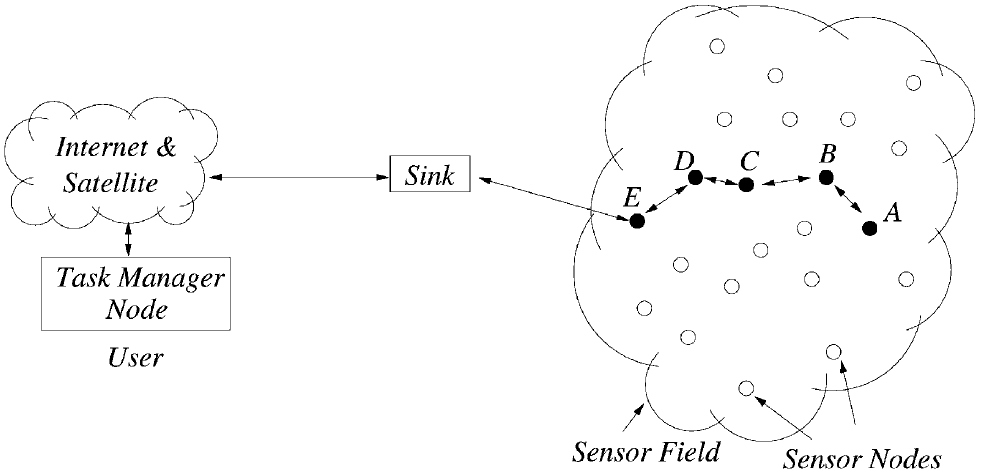
\includegraphics[scale=0.5]{Chapters/Figures/sensor_nodes_in_sensor_fields.png}
      \label{fig:sensor_nodes_in_sensor_fields}
\end{figure}

\subsection{Communication Architecture}
\label{subsec:wsn_communication_architecture}
The most common architecture for \glsxtrshort{WSN} follows the OSI model. The \glsxtrshort{WSN}
communication architecture is, however, only composed by five of the seven layers of the OSI
model: the application layer, the transport layer, the network layer, the data link layer
and the physical layer. It also is composed by three cross plane layers: the power management
plane, the mobility management plane and the task management plane, as shown in
Figure~\ref{fig:wsn_architecture}.

\begin{figure}[H]
      \caption{\glsxtrshort{WSN} Communication Architecture \cite{Akyildiz2002}}
      \centering
      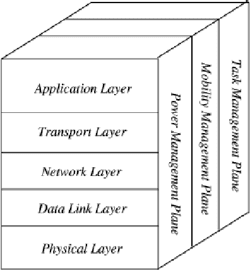
\includegraphics[scale=0.5]{Chapters/Figures/wsn_architecture.png}
      \label{fig:wsn_architecture}
\end{figure}

The five layers above mentioned work together to ensure the data is properly transmitted to
the network, each with a specific functionality \cite{Akyildiz2002, Matin2012}:
\begin{description}
      \item[Application Layer] provides to the end user an interface that he can interact with.
            Depending on the sensing tasks there are various types of application software that can
            be built.
      \item[Transport Layer] ensures the transportation of data in a reliable and orderly manner,
            even if the network suffers disruptions.
      \item[Network Layer] maps to where the data supplied by the transport data should go to
            next.
      \item[Data Link Layer] is responsible for confirming that the data transmitted is
            reliable and the transmission itself is efficient and secure. The main tasks of the
            data link layer are: 1) reducing the data received from the network layer into frames;
            2) find and correct errors in the frames, when possible; otherwise, discard them; 3)
            multiplexing of data streams; 4) \Gls{MAC}
      \item[Physical Layer] addresses the need for a simple but robust modulation, transmission
            and receiving techniques.
\end{description}

The management plane main roles are to include managing the network and optimize the sensor
nodes performance to improve the overall effectiveness of the network, considering the
advantages acquired by all sensor nodes working together. Each of these planes manages
a specific area \cite{Akyildiz2002}:
\begin{description}
      \item[Power Management Plane] manages how the sensor node uses its power, choosing when to
            turn off its receiver to save energy or to keep it from receiving repeated messages. It
            also informs its neighbours when it reaches a low power mode.
      \item[Mobility Management Plane:] keeps track of the sensor nodes neighbours and always
            distinguishes a route back to the user.
      \item[Task Management Plane:] administers the periodicity and schedule that each node needs
            to maintain in order to perform their sensing tasks based on their power dependency and
            task requirements.
\end{description}

\subsection{Network Topologies}
\label{subsec:network_topologies}
There are several different topologies \cite{Lewis2004, Yadav2012} regarding the connection
between nodes and their message exchange routes. In the Figure~\ref{fig:network_topologies} it
is possible to observe representations to the following topologies:
\begin{description}
      \item[Star Topology:] all nodes are connected to only one node, the coordinator. This
            means every node will communicate via this central node and every node that requests
            to enter this network will have to send its information to the coordinator, which
            will then send it to the other nodes. The principal limitation of this topology is
            that if the coordinator malfunctions the whole network will fail.
      \item[Ring Topology:] all nodes are equal connected, having no coordinator. Contrarily
            to the star topology, if a single link is broken the whole network will fail.
      \item[Bus Topology:] all nodes broadcast their messages using the bus. Each message
            has a header with the destination address so that every node can see if the message
            is for them or another node. This topology is passive, since the nodes are not
            responsible for retransmitting messages.
      \item[Tree Topology:] similar to the star topology where the coordinator is the tree root, on
            the other hand the nodes at different levels of hierarchy are connected to sub-coordinators
            that lead to the root \cite{Shrestha2007}. In this topology, as in the star topology, if
            the coordinator malfunctions, the whole network will fail. However, differently from
            the star topology, will also have problems if a sub-coordinator fails as it will lead
            to the failure of every subordinate node.
      \item[Fully Connected Topology:] every node is connected to every other node. This will
            lead to a routing problem when dealing with large networks.
      \item[Mesh Topology:] the nodes are generally identical, so the mesh connections are
            commonly referred as peer-to-peer connections. However, even though the nodes are
            generally identical some of them can be assign as coordinators that take additional
            functions and if one of these coordinators stops working, another just takes over his
            work. An interesting aspect of this topology is that the communication can be
            done between any two nodes in close proximity, which makes this topology quite
            robust to the failure of nodes or links, since the messages can use other routes to be
            delivered, and it is quite efficient for large scale networks.
\end{description}

\begin{figure}[H]
      \caption{Network Topologies \cite{Lewis2004}}
      \centering
      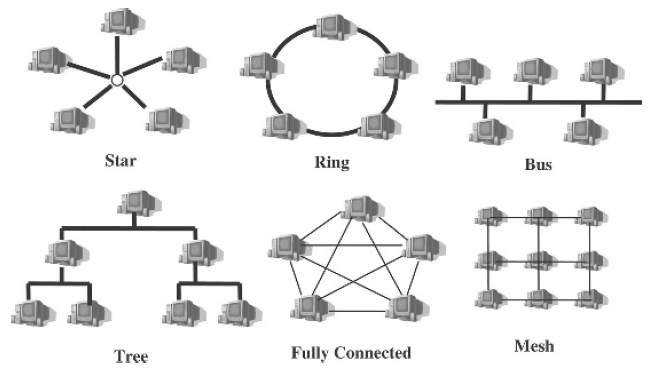
\includegraphics[scale=0.7]{Chapters/Figures/network_topologies.png}
      \label{fig:network_topologies}
\end{figure}


\subsection{Wireless Technologies}
\label{subsec:wsn_wireless_technologies}
To build a wireless network we need to consider the usage of wireless technologies, and their
characteristics and limitations. There are a multitude of technology alternatives available,
we will briefly examine six possibilities and later compare them in the Table~\ref{table:1}
%wifi is WLAN, bluetooth & zigbee are WPAN, lora & sigfox are LPWAN
\begin{description}
      \item[WiFi] - \Gls{WiFi} is a highly popular technology used to implement \Gls{WLAN},
            most commonly
            known for connecting smartphones and portable computers to the Internet without
            the usage of a physical connection \cite{Sidhu2007}. It uses \glsxtrshort{RF} to
            rapidly transmit data over short distances \cite{Khan2016}. However, for this
            technology to function it is necessary to already exist a \glsxtrshort{WiFi}
            network at its location \cite{Nelson2020}.
      \item[Bluetooth] - Bluetooth is a technology used to implement \Gls{WPAN},
            widely recognized for connecting multiple devices with each other,
            such as wireless computer mouses, headphones, computers and other \cite{Wang2021}.
            Similarly to \glsxtrshort{WiFi}, it transmits data over short distances, however
            the speed of these transmissions is very low. The most commonly network topology
            of Bluetooth is the piconet, where a Bluetooth device acts as the master and up to
            seven active devices act as slaves. The slaves can only communicate with the master,
            with point-to-point communication \cite{Cope2017, Lee2007}.
      \item[ZigBee] - ZigBee is a technology used to implement \glsxtrshort{WPAN}. Its name
            came from the way bees fly in zigzag, which is similar to
            the way nodes communicate in a mesh network. This technology is low cost, low
            complexity and low power, which makes it ideal for \glsxtrshort{WSN}. It has two
            different methods for access, the beacon enabled, that allows every node to send
            messages to the network whenever the channel is unoccupied, and the non beacon
            enabled, that only allows sending and receiving messages on a predefined time
            period \cite{Kaushal2014}. A ZigBee network has three types of devices: the
            coordinator, that creates and adjusts the network; the routers, that forward the
            data between the nodes; and the end devices, which cannot forward data from other
            nodes, only produce or consume it \cite{Costa2018, Ramya2011}. Besides the mesh
            topology, it is also ZigBee also supports the star and the tree topologies, as
            demonstrated in the Figure~\ref{fig:zigbee_topologies}, where the red nodes
            represent the coordinators, the blue nodes represent the routers and the orange
            nodes represent the end devices.
            \begin{figure}[H]
                  \caption{ZigBee Topologies \cite{Kaushal2014}}
                  \centering
                  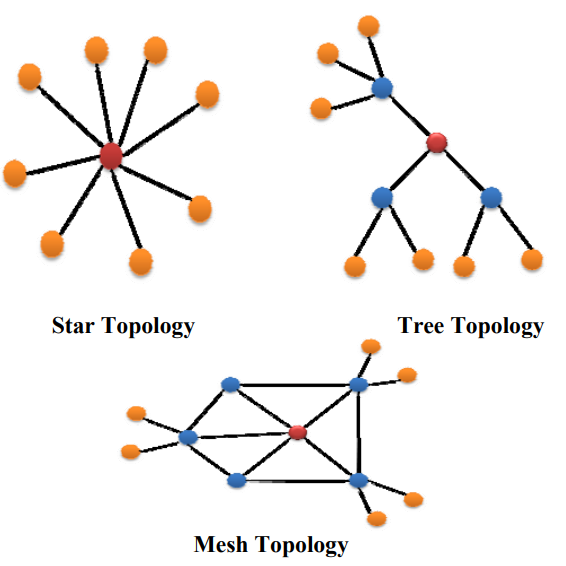
\includegraphics[scale=0.6]{Chapters/Figures/zigbee topologies.png}
                  \label{fig:zigbee_topologies}
            \end{figure}
      \item [NB-IoT] - \Gls{NB-IoT} is part of the \Gls{LPWAN} class of technologies. It is a
            type of cellular network developed to support low power and low cost devices in a
            long range area \cite{Beyene2017}. NB-IoT uses the \Gls{LTE} communication
            protocol, reducing some of its functionalities to minimize the power consumption,
            such small and infrequent message transmissions, as well as not implement features
            not needed for this types of networks \cite{Mekki2018}, like radio quality measures.
      \item[LoRa] - \Gls{LoRa} is part of the \glsxtrshort{LPWAN} class of technologies. It is a low
            power, long range and low data rate technology, which
            makes it a great choice for applications such as environmental monitoring, smart
            healthcare, industry, among others. This technology has been standardized by
            adding a \glsxtrshort{MAC} layer protocol, the \Gls{LoRaWAN}. The \glsxtrshort{LoRa}
            network has four basic elements: the LoRa nodes or end devices, the gateways, the
            network server and the application servers. The LoRa nodes or end devices are all
            the sensor nodes in the network. The gateways create the connection between end
            nodes and the network server. The data transmitted from each end node to each
            gateway is propagated using LoRa and LoRaWAN technologies, while the data propagated
            from the gateways to the network server uses Ethernet, cellular, satellite or
            Wi-Fi technologies. Then, the network server filters the data received from the
            gateways, perform security checks, adaptive data rates, and so forth, and, finally,
            sends an acknowledge back to the gateway and decides which application server
            receives that specific data and sends it. Lastly, the application server receive
            the data from the network server\cite{Carvalho2017, Devalal2018}.
            \glsxtrshort{LoRaWAN} is based on the star topology, shown in the Figure~\ref{fig:lora_topology},
            a topology that consumes a significant lower amount of power than other types of
            topologies, namely the mesh topology. The typical network consists of a star-of-stars
            topology, where the network is divided into cluster, each cluster containing multiple
            end devices and a gateway \cite{Aslam2019}.
            \begin{figure}[H]
                  \caption{LoRa Topology \cite{Devalal2018}}
                  \centering
                  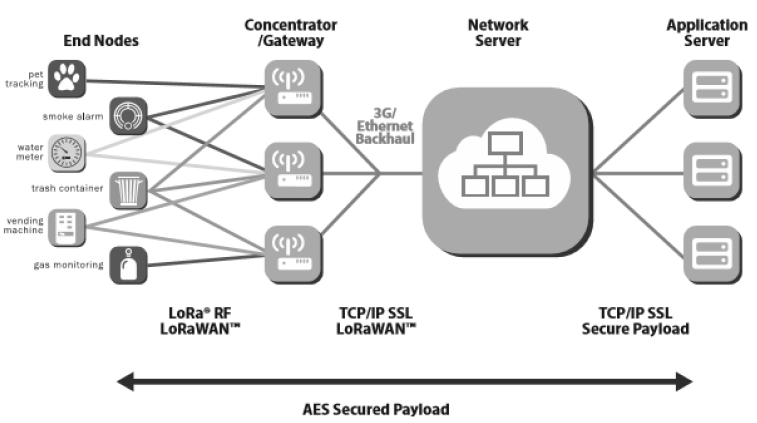
\includegraphics[scale=0.7]{Chapters/Figures/lora topology.png}
                  \label{fig:lora_topology}
            \end{figure}
      \item[Sigfox] - Sigfox, like \glsxtrshort{LoRa}, is part of the \glsxtrshort{LPWAN} class
            of technologies. It is also a low power, long range and low data rate technology.
            In Sigfox the network elements are equal to the ones of \glsxtrshort{LoRa}, however,
            the topology employed is a simple star topology, represent in the
            Figure~\ref{fig:sigfox_topology}. Contrarily to \glsxtrshort{LoRa}, Sigfox uses
            \Gls{D-BPSK} modulation, which only allows for the transmission of 4, 8 or 12 bytes
            messages with a bandwidth of 100Hz and speed of 100bps in Europe and it also only
            lets the transmission of 140 messages per day.
            \begin{figure}[H]
                  \caption{Sigfox Topology \cite{Petrariu2021}}
                  \centering
                  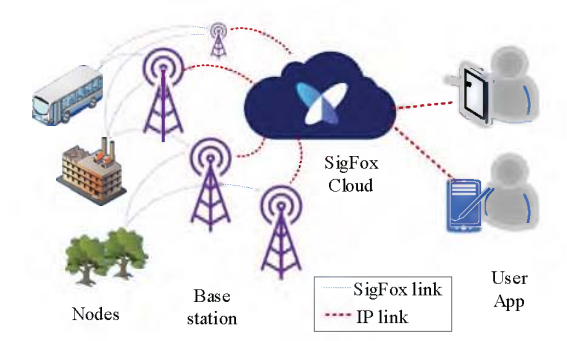
\includegraphics[scale=0.7]{Chapters/Figures/sigfox topology.png}
                  \label{fig:sigfox_topology}
            \end{figure}
\end{description}

\begin{table}[H]
      \centering
      \tiny
      \setlength\extrarowheight{5pt}
      \begin{tabular}{|c||c|c|c|c|c|c|c|}
            \hline
                      & \glsxtrshort{WiFi} 6 & Bluetooth 5.2 & ZigBee  & \glsxtrshort{NB-IoT}      & \glsxtrshort{LoRaWAN} & Sigfox \\
            \hline\hline
            \makecell[ct]{Frequency                                                                                                 \\Band} & \makecell[ct]{2.4GHz,\\5GHz,\\6 GHz}      & 2.4GHz   & \makecell[ct]{2.4GHz (global),\\868MHz (Europe),\\915MHz (America)}        & \makecell[ct]{Licensed \glsxtrshort{LTE}\\frequency bands} & \makecell[ct]{Unlicensed\\ISM bands}    &     \makecell[ct]{Unlicensed\\ISM bands}                                                                                           \\
            \hline
            \makecell[ct]{Max Data                                                                                                  \\Rate}     & 9.6Gbps             & 3Mbps        & \makecell[ct]{250kbps at 2.4GHz,\\20kbps at 868MHz,\\40kbps at 915MHz} & 200kbps &  290bps-50kbps                      &   100 bps     \\
            \hline
            Range     & max 300m             & 10m           & 10-100m & \makecell[ct]{1.5km urban                                  \\-\\20-40km rural}    & \makecell[ct]{2-5km urban          \\15km suburban\\45km rural}                      & \makecell[ct]{3-10km urban\\-\\30-50km rural}       \\
            \hline
            Bandwidth & 20-160MHz            & 1MHz          & 2MHz    & 200khz                    & 125KHz-250KHz         & 100Hz  \\
            \hline
            \makecell[ct]{Power                                                                                                     \\Consumption} & High                 & Low           & Low  &      Low           &    Low                  &     Low   \\
            \hline
            \makecell[ct]{Network                                                                                                   \\Topology}  & \makecell[ct]{Infrastructure\\(ad hoc also\\ available)}         & Piconet       & \makecell[ct]{Mesh,\\Star,\\Tree (peer-to-peer)}  &   Star   & Star-of-stars                  &   Star     \\
            \hline
      \end{tabular}
      \caption{Wireless Technologies Comparison \cite{Abdallah2020, Carvalho2017, Khan2016, Khorov2018, Oughton2021, Ramya2011, Zhang2018}}
      \label{table:1}
\end{table}

The six above described wireless technologies have different strengths and limitations, which
makes them more suitable for diverse types of applications. Since this work's problem is related
to multiple sensor nodes dispersed in a vast area, it is important to use a technology with
low power consumption and wide range, such as the \glsxtrshort{LPWAN} technologies. In the
Figure~\ref{fig:LPWAN_comparison} it is possible to observe the key advantages of each of these
technologies.

\begin{figure}[H]
      \caption{\glsxtrshort{LPWAN} Comparison \cite{Mekki2018}}
      \centering
      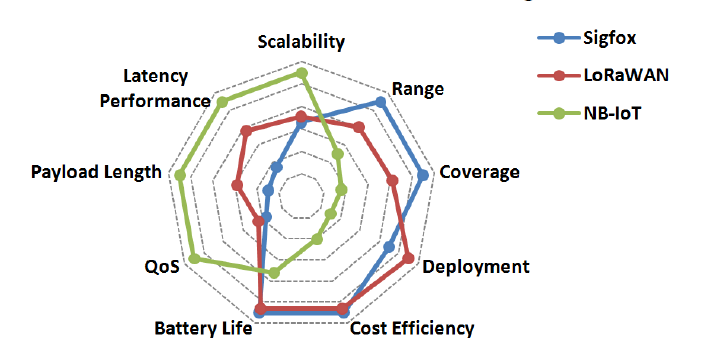
\includegraphics[scale=0.7]{Chapters/Figures/sigfox_nb-iot_lorawan_comparison.png}
      \label{fig:LPWAN_comparison}
\end{figure}

\subsection{Gossip in WSNs}
\label{subsec:gossip_in_wsns}
One of the main purposes of a sensor node is to transmit the data it has collected, via
the sensors, to the sink. The route chosen by these nodes has a significant impact on the
overall operation of the system, therefore various protocols were studied in \cite{Akkaya2005}
to understand which of these would better conduct this task.

As presented previously, in the Section~\ref{sec:gossip_protocols}, during the execution of a
gossip protocol each node only transmits its messages to \textit{t} randomly selected nodes
and not the whole network, as in the flooding protocol. This characteristic ensures that every
node executing a gossip protocol will only have a single copy of the packet to be sent, which
addresses one of the shortcomings of the flooding protocol, the implosion, this is, the nodes
receiving the same information twice \cite{Akkaya2005}. However, this will lead to delays in
the dissemination of the data which may be an important factor for some applications of the
network.

% %TODO: give examples of these protocols in wireless networks
% \subsubsection{Spawn}


% \subsubsection{SIG}

% \subsubsection{GSP}


\subsection{Applications}
\label{subsec:wsn_applications}
Due to the fact that the sensor nodes in a \glsxtrshort{WSN} may collect distinct types of
data, based on sensing task and the sensor itself, there are many applications and
subsequentially many are areas of expertise in WSR. These areas may be related to health, the
military, home, environmental, commercial and many more. For this thesis it is more impactful
to learn about some of the applications in the tracking area, per example, \nameref{subsubsection:zebranet}
and \nameref{subsubsection:wireless_tracking}.

\subsubsection{ZebraNet}
\label{subsubsection:zebranet}
One of the most revolutionary applications of \glsxtrshort{WSN} is the ZebraNet\cite{Juang2002}, a method
developed to track wildlife, specifically, zebras, for biology research, using a mobile base
station. The ZebraNet collects logged data from tracking collars, transported by the
animals, and afterward it transmits this data back to the researchers.

The ZebraNet project focused on addressing some of the problems observed from previous
studies of collecting data from wildlife. One of the main obstacles was using
satellites to transport the data. The process of uploading data to satellites is slow and
power consuming. Moreover, the data download from the satellite to the researchers is
charged by the bit, which restricted the amount of data collected. Furthermore, these
systems used batteries without solar panels, which would eventually end, and had to be
recovered and recharged, losing enormous amounts of data in process.

This project was developed in a wide area, with hundreds or thousands of square kilometres,
and lasted a year without direct human interaction. It used \glsxtrshort{GPS} technology to
obtain the position of the animals every three minutes, and also collected detailed activity
logs every hour during three minutes. Considering there is no fixed antennas or cellular
telephone service, the system used an ad hoc peer-to-peer routing to transport the data from
one animal to the next towards a mobile base station, when it was in close proximity.

During the development of this project there were some design limitations to consider, due to
the fact that each node would be transported by an animal, its weight and size was immediately
limited. And since the nodes are difficult to retrieve, the device had to have a durable
battery life \cite{Zhang2004}. Subsequentially, most of the weight would be occupied by the
battery and the GPS, leaving a small space for the storage, which meant that there was a
small space for redundant messages in this protocol. Lastly, it was crucial to consider the
impact of the number and size of data transmissions required, as well as the range of these
transmissions and the amount of storage available to keep the activity logs.
During the course of years there were developed many hardware alternatives \cite{Zhang2004}.

The first protocol contemplated to undertake the ZebraNet communication between the nodes and
the base station was flooding. The flooding protocol disseminates the data to all nodes
available, which will eventually lead to a high percentage of the information to reach the
base station even if it is only in contact with a few of the nodes. While flooding has high
reliability, it also has high overhead, which increases the need for a larger amount of
storage and will eventually tend to a higher network bandwidth and therefore energy required.

It was then considered a protocol that took in consideration the previously used communication
patterns. It associates a hierarchy level to every node based on his past success in delivering
data to the base station. If a node had a high level it is probable that he is still in range
of the base station or of another node close to it. Every node has to have knowledge of his
own hierarchy level and when he scans for neighbours it requests their hierarchy levels. The
nodes send their collected data to the neighbour with the highest hierarchy level. The hierarchy
level increases when a node is in range of the base station and decreases when it is not in
range for a period of \textit{D} scans, this means that if \textit{D} is three and the node is
not in range of the base station during three consecutive scans his level will decrease.
Initially all nodes start with the lowest hierarchy level, zero. The overall success of this
protocol vastly depends on the mobility of the nodes and the base station. Since it is based
on previously acquired data, with rapid changes of locations on either the base station or
the nodes the success rate will be low.


\subsubsection{Wireless Tracking}
\label{subsubsection:wireless_tracking}
Wireless tracking is an application of \glsxtrshort{WSN} widely used for wildlife monitoring,
since it allows the remote monitorization of moving objects, or in this particular case,
animals.

To track an object the sensor nodes detect its location and sends this information to the end
user. There are mainly two options to accomplish this: using only a single node or multiple
nodes working collaboratively. Using multiple nodes is an overall better choice, since it leads
to higher accuracy and lower power consumption comparably to using a single node \cite{Ez2016}.

To conserve energy it is common to keep only the sensor nodes closest to the target in active
mode, while the other nodes remain inactive until the target approaches them

To achieve an efficient target tracking performance it was developed countless methods,
contemplating the challenges existent with using \glsxtrshort{WSN}, discussed furthermore in
the Section~\ref{subsec:wsn_limitations}. These methods take into account the continuous
localization of mobile nodes over time, determine their speed at each moment and often use
their known former localization to improve accuracy \cite{Kumar2017}.

There are two main types of target tracking approaches according to \cite{Ramya2012} authors:
\begin{enumerate}
      \item Hierarchical Networks - the nodes communication follows a mesh based topology,
            thoroughly explain in the Section~\ref{subsec:network_topologies}, using multi hop
            radio connectivity. This enables the communication between two nodes that are not
            in a direct communication range, by forwarding their messages through other nodes
            in their ranges until the messages achieve their final destination. There are four
            methods of tracking belonging to the these networks: Tree-Based Target Tracking,
            Cluster Based Target Tracking, Hybrid method and Activation method.
            \begin{enumerate}
                  \item Tree Based Target Tracking - the nodes are organized in a hierarchical
                        tree structure or represented as a graph, where the vertices represent
                        the nodes and the edges the connections between two nodes that can
                        communicate directly.

                        The node that find the target communicate with all the rest of the
                        nodes in the network and collectively select one node to be the root.
                        The root node will gather the information from all other nodes via a
                        distributed spanning tree. If the root gets far away from the target,
                        the spanning tree will have to be reconstructed, leading higher energy
                        consumption. For this reason there were proposed several algorithms,
                        such as \glsxtrshort{STUN} \cite{Kung2003}, \glsxtrshort{DCTC} \cite{Zhang2004},
                        \glsxtrshort{DAT} \cite{Lin2006}, \glsxtrshort{DOT} \cite{Tsai2007}, \glsxtrshort{OCO}
                        \cite{Tran2006}.
                  \item Cluster Based Target Tracking - the network is organized into clusters,
                        and each cluster is composed by a cluster head and members nodes.
                        In this type of target tracking, the nodes, usually, surround the target
                        and collaborate to estimate its location.

                        There are three types of cluster based approaches, the static
                        clustering, the dynamic clustering and the space-time clustering.
                        \begin{enumerate}
                              \item In static clustering, the attributes of each cluster are defined once,
                                    when the network is deployed. This may lead to some disadvantages, since
                                    the nodes cannot change clusters as needed. For example, if a cluster
                                    head node fails, the entirety of that cluster becomes useless. Also
                                    nodes from different clusters cannot communicate or collaborate in
                                    data processing.
                              \item In dynamic, contrarily to static clustering, nodes do not statically
                                    belong to a specific cluster, removing some of the previous limitations
                                    of static clustering. In dynamic clustering when a node detects the target,
                                    and it has enough battery and computational power, it volunteers to
                                    act as cluster head. The cluster head will be the only node active in
                                    close proximity with the target.
                              \item In space-time clustering, uses algorithms such as
                                    the closest point of approach, to declare which node is the
                                    cluster head. In \glsxtrshort{DSTC} \cite{Phoha2005} it is declared that the cluster
                                    head is the node that is in close proximity with the most other
                                    nodes.
                        \end{enumerate}
                  \item Hybrid Method - Hybrid methods are tracking algorithms that provide
                        solutions for multiple types of target tracking, some examples of
                        these methods are \glsxtrshort{DPT} \cite{Yang2003}, \glsxtrshort{DCAT}
                        \cite{Chen2004} and \glsxtrshort{HPS} \cite{Ramya2012}.
                  \item Activation Based Method - In this methods, it is considered which nodes
                        should be active and which can be asleep, if they are far from the
                        target, for example. Some of these methods are the Naive activation
                        based tracking \cite{Pattem2003}, the Randomized activation \cite{Bisnik2006},
                        the Selective activation based on prediction \cite{Ramya2012} and the
                        \glsxtrshort{DA} \cite{Zahedi2010}
            \end{enumerate}
      \item Peer-to-peer Networks - in tree and cluster-based target tracking there is a lack of
            robustness to failures, since if the root or cluster head fail the whole system
            might fail as well. In peer-to-peer \glsxtrshort{WSN}, since it relies on single
            hop communications, this problem does not occur.
\end{enumerate}


\subsubsection{Yggdrasil}
\label{subsubsection:Yggdrasil}
Wireless ad hoc networks often use cloud-based solutions to process and storage the data
collected by the sensor nodes, however, for large scale networks this implies a large volume
of data being relayed and processed, leading to potential delays. An approach to resolve this
situation is to process and storage the collected data directly in the edge nodes. The edge
nodes should also be able to connect with each other, sharing the data. To implement a system
with these characteristics it was developed Yggdrasil.

Yggdrasil \cite{Costa2018} is framework and middleware that provides support for developing
and executing distributed protocols and applications in wireless ad hoc settings. It combines
an event-driven programming model and a multi-threaded execution environment to deal with
possible concurrency issues derived from the distributed protocol.

In Yggdrasil each protocol has its own internal state that can change as events occur. Each
protocol can generate events to process himself or to deliver to another protocol (or
application). There are four types of events that change the execution of the protocols:
messages, that can be transported between processes; timers, that serve to inform about the
execution of a time-driven task or that a local timeout occured; requests/replies, enables
direct one-to-one interaction between protocols in the local process; and notifications,
enables indirect one-to-many interaction between protocols in the local process. Each protocol
(and application) has an event queue with the events created by them and the ones created by
other protocols, to easly relay events from the protocol that created them to the protocol (or
application) to which they should be delivered to.


\subsubsection{\Gls{MiRAge}}
\label{subsubsection:mirage}
\glsxtrshort{MiRAge} \cite{Costa2018} is a protocol that employes a self-healing spanning
tree to efficiently support aggregation.

In MiRAge all nodes compete to be the root of the tree. This competition uses an assigned
identifier for each node and a sequence number, timestamp, maintained by the root node.
If the sequence number does not increase, this means that the root node suffered a fault,
making the tree incorrect. A tree is considered correct if the root is non-faulty. When
dealing with two correct tree, the winner will be the one who's root identifier is lower.
While constructing the spanning tree the goal is to obtain a dominating tree, this is, a
single spanning tree that covers the whole network to provide an efficient and reliable form
to aggregate values. This dominating tree will be the correct tree with the lowest identifier.

In MiRAge the nodes are unware of who are their children or parent in the tree, since they
relay to their neighbours alike the resulting aggregated value, not taking into consideration
their contribution. They need, however, to remeber the links of the tree they belong to. This
is obtained by keeping the node's identifier and a status, active for nodes in the same tree
and passive for nodes in other trees.

Each node also keeps a local aggregation value and its current estimation of the aggregation
result. The estimated result is constantly being updated with an aggregation function that
uses the nodes received estimations performed by the neighbours belonging to the same tree.
After this update, the node sends a message, through one hop broadcast, containing a reversed
calculation of the estimated result, by removing the contribution of a neighbour. This
calculation will be tagged alongside the neighbours identifier, forming a tuple for each
neighbour. When a node receives one of these messages it updates the information of the sender.
If it is the first message received by this sender it sets his status to passive.

When propagating aggregation information the nodes also relay some information about the tree
that they belong to as well as their position on it. With this information it is possible to
ensure that the dominating tree covers all nodes, that the tree is healed if there are failures
and that a node is not permited to connect to a tree whose root has failed.


\subsection{Limitations}
\label{subsec:wsn_limitations}
There are multiple limitations that need to be considered while creating a \glsxtrshort{WSN}
\cite{Akyildiz2002, Matin2012}:
\begin{itemize}
      \item \textbf{Fault Tolerance} - the sensor nodes can fail due to lack of power, hardware
            problems or physical damage, contemplating the harsh environments they are exposed to
            and their own fragility. Therefore, the protocols employed in the sensor network
            need to possess the ability to quickly identify any malfunctions and possess the
            robustness necessary to sustain the network's overall functionality, even with a large
            number of failures.
      \item \textbf{Scalability} - the sensor networks might have hundred, thousand or even
            millions of nodes. Therefore, the protocols employed in these sensor networks need to
            be scalable to these levels and maintain a tolerable efficiency level.
      \item \textbf{Production Costs} - since a sensor network is composed by a large number of
            nodes it is important that this value is quite small, ideally much lower than US\$1.
      \item \textbf{Hardware Constraints} - a sensor node is usually constituted by a sensing
            unit, a processing unit, a transmission unit and a power supply, as represented in
            Figure~\ref{fig:sensor_components}. Additionally, it may be necessary to add some
            extra components, as per example a localization system. These need to consider the
            extra costs, the power consumption it will lead to and finally, the space available
            in the node.
            \begin{figure}[H]
                  \caption{Sensor node typical architecture \cite{Akyildiz2002}}
                  \centering
                  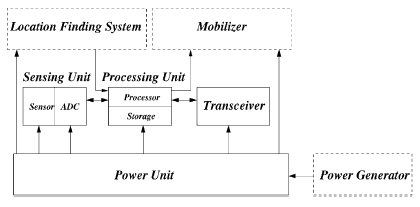
\includegraphics[scale=1]{Chapters/Figures/sensor_components.png}
                  \label{fig:sensor_components}
            \end{figure}
      \item \textbf{Sensor Network Topology} - energy consumption is the main obstacle regarding
            \glsxtrshort{WSN} performance and efficiency. To combat this problem it has been
            researched numerous algorithms, protocols and techniques, being topology maintenance
            one of the most important to reduce energy consumption.
      \item \textbf{Transmission Media} - most communication networks use \Gls{RF} to connect
            the nodes wirelessly. There are, however, other ways of connection, using optical or
            infrared communication. Both optical and infrared communication require a line of
            sight between the sender and the receiver. However, the infrared communication has
            the advantage of being less affected by other electronic devices.
      \item \textbf{Power Consumption} - derived from the node size and the, sometimes,
            impossibility to recharge its battery, the lifetime of a node depends entirely
            on the management of this resource. Therefore, it is of the utmost importance to
            carefully consider the power consumption while developing the software and hardware
            designs.
      \item \textbf{Environment} - the nodes may be deployed in various different environments,
            ranging from a rural area to the bottom of the ocean. Therefore, it is necessary to
            consider the environment implications on the network nodes, in order to protect them
            and ensure they can perform their function properly.
\end{itemize}


\subsection{Discussion}
Throughout this Section it has been discussed how \glsxtrshort{WSN} generally work,  some of the
different wireless technology available, some examples of how to operate gossip protocols in
\glsxtrshort{WSN}, a few of this type of networks applications, namely ZebraNet, Wireless Tracking,
Mirage and Yggdrasil, and their limitations.

To building a \glsxtrshort{WSN} it is of the upmost importance to consider the necessity for
low energy consumption devices, which will have a great impact while deciding the hardware
and software designs for our sensor nodes. It is essential to have a protocol for the
communication between the nodes both reliable and power efficient.

The ZebraNet application is very important for our problem resolution since it deals with the
collection of information in a similar situation to the one we encounter in the Coitadinha
farm, where there are mobile nodes carried by animals and potentially mobile base stations
as well. Just as in ZebraNet, we want to have an infrastructure-less network.



\section{Existing Commercial Solutions}
\label{sec:existing_commercial_solutions}
Throughout the last few years there have been developed diverse solutions for problems similar
to ours. Every solution has different characteristics, as represented in the Table~\ref{table:2},
where it is made a comparison between seven solutions, we found interesting for this work.

\begin{table}[t]
      \tiny
      \centering
      \setlength\extrarowheight{10pt}
      \begin{tabular}{|c|c||c|c|c|c|c|c|c|c|c|}
            \hline
                                                                    &                       & \multicolumn{2}{|c|}{Digital Matter} &            &            &            &            &            &                     &                         \\
            \hline
                                                                    &                       & \makecell[ct]{Oyster                                                                                                                                  \\Edge \cite{Oyster}}                         & \makecell[ct]{Yabby\\Edge \cite{Yabby}} & \makecell[ct]{Digitanimal\\\cite{Digitanimal}} & \makecell[ct]{Chipfox\\\cite{Chipfox}}    & \makecell[ct]{IoT Factory\\\cite{Iotfactory}} & \makecell[ct]{Nofence\\\cite{Nofence}}    & \makecell[ct]{Vence\\\cite{Vence}}      & \makecell[ct]{eShepherd\\\cite{Eshepherd}}  & \makecell[ct]{Halter\\\cite{Halter}}     \\
            \hline\hline
            \multirow{6}{*}{\rotatebox[origin=c]{90}{Applications}} & \makecell[ct]{Virtual                                                                                                                                                         \\Fence} & \makecell[ct]{Alert\\ in App}                         &  \makecell[ct]{Alert\\ in App} &  \makecell[ct]{Alert\\ in App} &  \makecell[ct]{Alert\\ in App} &             & \makecell[ct]{Audio +\\Eletric} & \makecell[ct]{Audio +\\Eletric} & \makecell[ct]{Audio +\\Eletric} & \makecell[ct]{Audio +\\Eletric} \\
            \cline{2-11}
                                                                    & Tracking              & \textbf{X}                           & \textbf{X} & \textbf{X} & \textbf{X} &            & \textbf{X} & \textbf{X}          & \textbf{X} & \textbf{X} \\
            \cline{2-11}
                                                                    & Axis Angles           & \textbf{X}                           &            &            &            &            &            &                     &            &            \\
            \cline{2-11}
                                                                    & Health Issues         &                                      &            & \textbf{X} &            & \textbf{X} &            & \textbf{X}          &            & \textbf{X} \\
            \cline{2-11}
                                                                    & Temperature           &                                      &            & \textbf{X} &            &            &            &                     & \textbf{X} & \textbf{X} \\
            \cline{2-11}
                                                                    & Real-time             & \textbf{X}                           & \textbf{X} & \textbf{X} & \textbf{X} & \textbf{X} & \textbf{X} & \textbf{X}          & \textbf{X} & \textbf{X} \\
            \hline
            \multirow{5}{*}{\rotatebox[origin=c]{90}{Technologies}} & WiFi                  & \textbf{X}                           & \textbf{X} &            &            &            &            &                     &            & \textbf{X} \\
            \cline{2-11}
                                                                    & Bluetooth             & \textbf{X}                           &            & \textbf{X} &            & \textbf{X} & \textbf{X} &                     &            &            \\
            \cline{2-11}
                                                                    & Cellular              & \textbf{X}                           &            &            &            &            & \textbf{X} & \textbf{X}          & \textbf{X} &            \\
            \cline{2-11}
                                                                    & LoRaWAN               &                                      & \textbf{X} &            &            & \textbf{X} &            &                     &            & \textbf{X} \\
            \cline{2-11}
                                                                    & Sigfox                &                                      &            & \textbf{X} & \textbf{X} &            &            &                     &            &            \\
            \hline
            \multirow{2}{*}{\rotatebox[origin=c]{90}{Backend}}      & Cloud                 & \textbf{X}                           & \textbf{X} &            & \textbf{X} & \textbf{X} &            & \textbf{X}          & \textbf{X} & \textbf{X} \\
            \cline{2-11}
                                                                    & Private Server        &                                      &            & \textbf{X} &            &            & \textbf{X} &                     &            &            \\
            \hline
            \multirow{2}{*}{\rotatebox[origin=c]{90}{Network}}      & Peer-to-peer          &                                      &            &            &            &            &            &                     &            &            \\
            \cline{2-11}
                                                                    & Infrastructure        & \textbf{X}                           & \textbf{X} & \textbf{X} & \textbf{X} & \textbf{X} & \textbf{X} & \textbf{X}          & \textbf{X} & \textbf{X} \\
            \hline
            \multirow{2}{*}{\rotatebox[origin=c]{90}{Battery}}      & Duration              & 4.5years                             & 3years     & 1.5years   & 3years     & 1-2years   & no data    & 1-2years            & no data    & no data    \\
            \cline{2-11}
                                                                    & Solar Painel          &                                      &            &            &            &            & \textbf{X} &                     & \textbf{X} & \textbf{X} \\
            \hline
            \multirow{2}{*}{\rotatebox[origin=c]{90}{Price}}        & Per Collar            & 189.03€                              & 106.98€    & 189.95€    & 143.79€    & no data    & 303€       & \textasciitilde 33€ & 60-90€     & no data    \\
            \cline{2-11}
                                                                    & Infrastructure        & no data                              & no data    & no data    & 681.51€    & no data    & no data    & no data             & 5000€      & no data    \\
            \hline
      \end{tabular}
      \caption{Commercial Solutions Comparison}
      \label{table:2}
\end{table}

There are different applications available in each of these collars, such as:
\begin{enumerate}
      \item Tracking - provides information on where the cattle has been during a period of
            time, being this data collected every few minutes or every hour, depending on the
            collar;
      \item Real-time localization - which makes it possible to always know where all cows
            are at any moment;
      \item Virtual fencing - when available it is possible for the user to create a virtual
            barrier on an mobile application, and when an animal crosses this barrier it can
            either alert the user on the application, or force the cow to go back inside the
            fence with the usage of sound triggers first and if the cow continues to leave the
            enclosed area the collar delivers a low intensity shock to the cow \cite{Golinski2022}.
            This technique will teach the cattle to not cross the barrier as soon as they hear
            the initial sound delivered by the collar, so that they do not receive the shock;
      \item Health issues detection - some of these collars have other sensors embedded in them,
            such as heart rate monitorization, which allows the detection of health issues or
            imminent birth sooner;
      \item Temperature detection - similarly to the detection of health issues, some of the
            explored solutions are able to detect abnormal temperatures for cattle and report
            it to the user;
      \item Axis angles detection - the device with this feature allows to detect the angle
            presented by the device, which may be useful to better understand the cow's
            behaviour, for example detect if she is eating, drinking, sleeping, among others.
\end{enumerate}

\subsection{Discussion}
\label{subsec:commercial_solutions_discussion}
The current existent commercial solutions are quite helpful for this work, since they allow us
to compare the success and metrics of our future solution with the obtained by these collars,
that are already in the market.

However, they are not a perfect solution for our particular
problem due to their lack of peer-to-peer options for communication and expensive price.


\section{Cattle Production}
\label{sec:cows}
Some animals are known to form subgroups to perform their everyday tasks. In the case of
cows, these groups are called herds and they distinguish three main activities: resting,
grazing, and travelling. We will discuss next how cows behave.

\subsection{Cattle Behaviour in Herds}
\label{subsec:behaviour_herds}
The cows follow a hierarchical system, where the oldest cow is regularly the leader of the
herd. Scarcely, there is a younger, stronger, cow leading a group \cite{Harris2007}. This
leader can choose where the herd moves, having influence over the other cows that follow her.
This effect is more pronounced when the herd is travelling in comparison to when they are
grazing or resting \cite{Vsarova2010}.

A study was conducted that observed the interactions of cows during the course of two
years. During this research the authors reached some interesting conclusion about the proximity
demonstrated by these animals. It was found a correlation between the distance of neighbours
in a herd and the quantity of pasturage available. When there is abundant nourishment, the
herd are more compact, and the animals graze closer together \cite{Harris2007}.

\subsection{Diet Impact on Plant Communities}
\label{subsec:diet}
The diet of an animal has a profound impact on the quality of the products derived from it \cite{Araujo2014}.
Therefore, it is reasonably for farm owners to feed their cattle with natural vegetation, when
possible, instead of synthetic one.

In 2018, a study was conducted in the Netherlands that distinguished the dieting habits of
three species: cattle, bison, and horses \cite{Cromsigt2018}. During this study it was
discovered that the cattle eating habits, in a landscape without supplementary feeding,
consisted mostly on grass (around 80\%) and woody plants, twigs and leaves, (around 20\%). It
was supposed that the consume of woody plants was derived from the lack of grass during the
winter. Without the data from a similar study convened in Portugal, we can only presume that
with the more favourable climatic conditions the cattle would feed almost completely on grass.

A study was conducted on three ranches in Texas with the purpose of understanding the impact
of distinct types of grazing on the soil and vegetation. In the first ranch it was used the
multi-paddock technique, in the second one it was used light continuous grazing and in the
last one it was used heavy continuous grazing. With the multi-paddock method, the terrain is
divided in multiple smaller paddocks and regularly each herd rotates from one paddock to the
next. In the end, it was concluded that this type of grazing management is overall better for
the soil and vegetation that the light or the heavy continuous grazing methods \cite{Teague2011}

\subsection{Discussion}
\label{subsec:cow_discussion}
It is imperative to understand how cows behave to correctly develop a tracking system that
works for them and considers their behaviour, to minimize costs and ensure correct operations.

Comprehending the relation and the distance between individual cows and their neighbours is
of utmost importance for my future work, considering that the messages collected from each
cow will have to be disseminated using a peer-to-peer based protocol.

Furthermore, it is fundamental to consider in my next steps that the farm owners should be able
to shift the grazing location of the herds to obtain a wealthier vegetation and soil, leading
to overall better cattle.


\section{Summary}
\label{sec:summary}
In this chapter we exposed the already existing protocols and networks available to help us
develop our work.

We started by explaining the gossip protocols, as a reliable and scalable
solution for the dissemination of information, which is fundamental for our work as we will be
using a gossip-based protocol to relay the cows collected sensing information back to
the user without the usage of infrastructures.

We then discussed \glsxtrshort{WSN}, the way it operates, how to include gossip-based protocols
in this kind of networks, some of its applications and lastly the limitations that need to be taken
into consideration while dealing with these types of networks, specifically the need for low power
consumption options.

Later, we collected some information about the commercial solutions available and their pros
and cons and discussed the need for a new solution to resolve this works problem.

Ultimately, we gathered some information regarding cattle production, we researched how they
behave when they are in herds and the impact of their diet on the plant communities. This
information will be useful for the development of our prototype since it tells that it is
probable that cows walk together and that they follow a leader.

In the following chapter we will briefly describe the plan for the foreseen chapter of this
work and the timeline for it.